\documentclass[10pt, a4paper]{article}

\usepackage[utf8]{inputenc}
\usepackage[T1]{fontenc}
\usepackage{charter}
\usepackage{microtype}
\usepackage[margin=1in]{geometry}
\usepackage{changepage}
\usepackage{csquotes}
\usepackage{tikz}
\usetikzlibrary{arrows.meta, positioning, decorations.pathmorphing, patterns}
\usepackage{hyperref}

\renewcommand{\thesection}{\arabic{section}.}
\renewcommand{\thesubsection}{\arabic{section}.\arabic{subsection}.}

\hypersetup{
  colorlinks=true,
  linkcolor=black,
  urlcolor=black,
  citecolor=black,
  pdftitle={Mru: A Fault-Tolerant Operating System for Thousand-Year Autonomous Operation},
  pdfauthor={Will Binns},
  pdfsubject={Autonomous spacecraft software architecture for millennial-timescale operation},
  pdfkeywords={autonomous systems, fault tolerance, interstellar probe, graceful degradation, formal verification, operating systems}
}

\title{Mru\\[0.3cm]
\large A Fault-Tolerant Operating System for Thousand-Year Autonomous Operation}
\author{Will Binns \\ \small hello@wbnns.com}
\date{May 2026}

\begin{document}

\maketitle

% ===== ABSTRACT =====
\begin{adjustwidth}{0.5in}{0.5in}
\noindent\textbf{Abstract.}\quad No software system in human history has been designed to operate for centuries without human intervention. The longest-lived systems we have built---deep-space probes approaching fifty years of service, banking codebases approaching sixty---survive only through continuous human maintenance. An interstellar probe operating for 500 to 1{,}000 years cannot: its hardware is guaranteed to fail, its power to decline, its memory to corrupt, and the light-delay makes human guidance physically impossible. This paper introduces Mru, an open-source operating system that treats this physical decay not as an exceptional fault but as the governing design constraint. I formalize the stance as the \textit{Degradation-First Principle} and derive from it a layered architecture modeled on biological robustness: a minimal, formally verified interpreter, replicated across reconfigurable hardware, that executes behavior encoded as mutable data---the way DNA encodes behavior run by a replicated molecular interpreter. On this kernel I build hardware consensus among failing nodes, knowledge triage, autonomous science, bandwidth-starved communication, and bounded self-modification, validated in simulation grounded in published radiation, power, and failure models. I argue that designing software to outlive its makers is not speculation but a tractable engineering discipline---one the interstellar case makes unavoidable, and a growing class of terrestrial systems increasingly needs.
\end{adjustwidth}

% ===== 1. INTRODUCTION =====
\section{Introduction}

The Bracewell probe---an autonomous interstellar messenger that travels to a target star system and operates on arrival without instruction from its makers---was proposed more than six decades ago as a strategy for interstellar communication that does not depend on continuous two-way contact \cite{bracewell1960}. The propulsion required to send such a probe between stars remains beyond present capability. The \textit{software} required to keep one alive for the duration of the journey, however, can be designed, built, and validated today. It has simply never been attempted, because no terrestrial problem has ever demanded it.

The forcing scenario is unforgiving. The one-way light-time to even the nearest star system is measured in years, so round-trip guidance is impossible; every decision must be made locally \cite{muscettola1998}. The journey lasts centuries, over which cosmic radiation will flip bits, damage transistors, and accumulate ionizing dose in every component aboard \cite{baumann2005, normand1996}. The power source decays on a fixed physical schedule that no software can arrest. There are no updates after launch: every latent bug will eventually be reached, and every unhandled case will eventually occur. The probe must therefore be simple enough to run correctly for a thousand years and, at the same time, autonomous enough to make consequential scientific decisions about an environment no engineer could anticipate at launch.

It is worth measuring this against what humanity has actually built. The Voyager spacecraft, the longest-operating deep-space missions in history, have functioned for nearly half a century---but only with a standing team on Earth issuing commands, and on a radioisotope power source that has already declined to roughly half its launch output \cite{kohlhase1977}. The longest-lived software on Earth, the COBOL systems that still run banks and government agencies, have endured for some sixty years---but only through the continuous labor of human engineers patching, migrating, and nursing them along \cite{gao2016}. Remove the humans from either, and the system fails in years, not centuries. \textit{No artifact we have ever made survives unattended on the timescale Mru targets.}

This paper proposes that the obstacle is not fundamentally one of capability but of \textit{stance}. Conventional software is built on an implicit assumption of maintenance: that a human will eventually arrive to fix what breaks. Strip that assumption away and a different design discipline is required---one in which the system's own decay is the central fact around which everything else is arranged. I formalize this as the Degradation-First Principle and show that a coherent architecture follows from it. I name the system Mru, a contraction of \textit{Maru}---the suffix, from the character for ``circle,'' that is traditionally borne by seagoing vessels, connoting completeness and safe passage on a long voyage. The open-source reference implementation and its command-line interface are named \texttt{mru}. Mru is at once an operating system---a formally verified survival kernel and the resource management beneath everything else---and the layered software architecture of the autonomy stack that runs upon it.

% ===== 2. RELATED WORK =====
\section{Related Work}

Mru draws on several mature engineering and scientific traditions. No prior system unifies them under the constraint of unattended millennial operation, but each supplies a load-bearing component of the design.

\subsection{Spacecraft Longevity and Autonomy}

Deep-space missions have pushed operational lifetimes to unprecedented lengths and pioneered onboard fault protection and autonomy \cite{kohlhase1977}. The Remote Agent experiment aboard Deep Space~1 demonstrated that a spacecraft could plan, execute, and recover from faults without ground intervention \cite{muscettola1998}. Yet every flown system shares a common assumption: that a human operations team remains reachable across a light-delay of at most hours, able to upload new sequences and diagnose anomalies. Mru removes that assumption entirely.

\subsection{Deep-Space Power Systems}

Beyond the orbit of Jupiter, solar power is impractical, and the radioisotope thermoelectric generator (RTG) has been the only proven deep-space source \cite{bennett2006}. RTGs decay on the fixed schedule of their fuel: plutonium-238 has a half-life of 87.7 years, so after several centuries an RTG produces effectively no useful power. Small fission reactors of the Kilopower class offer higher output, and the KRUSTY experiment demonstrated a working uranium-fueled unit, but fuel remains finite \cite{gibson2017, poston2020}. Power, not computation, is the master constraint of any millennial mission.

\subsection{Fault-Tolerant and Reliable Computing}

The intellectual foundation of Mru's kernel is von Neumann's demonstration that arbitrarily reliable computation can be synthesized from unreliable components through redundancy and multiplexing \cite{vonneumann1956}. Triple modular redundancy formalized one practical realization \cite{lyons1962}, and the modern taxonomy of dependable computing distinguishes the faults, errors, and failures that such schemes must contain \cite{avizienis2004}. The Byzantine Generals problem established the limits of agreement when components may behave arbitrarily \cite{lamport1982}; I argue below that its adversarial threat model is the \textit{wrong} model for a probe whose nodes are damaged rather than malicious.

\subsection{Radiation Effects and Reconfigurable Hardware}

Single-event upsets, single-event latchups, and total ionizing dose are the physical mechanisms by which space radiation degrades electronics \cite{normand1996, baumann2005, schwank2008}. Field-programmable gate arrays (FPGAs) offer a uniquely valuable response: their configuration can be scrubbed to repair upsets and, more importantly, their logic can be re-placed onto surviving fabric as gates die---a capability with extensive flight heritage in high-reliability systems \cite{wirthlin2015}. This is the hardware substrate that makes graceful degradation physically real rather than merely aspirational.

\subsection{Memory, Information Theory, and Error Correction}

The durability of stored knowledge rests on the theory of error-correcting codes, beginning with Shannon's channel capacity and Hamming's first error-correcting construction \cite{shannon1948, hamming1950}. Reed--Solomon codes underpin durable storage \cite{reedsolomon1960}, while low-density parity-check and turbo codes approach the Shannon limit for communication at extreme signal-to-noise ratios \cite{gallager1962, berrou1993}. The physical durability of the storage medium matters as much as the code: non-volatile memories such as MRAM and FeRAM offer radiation tolerance and retention properties suited to long missions \cite{gerardin2010}. Periodic scrubbing of memory contents is itself a well-studied reliability technique \cite{saleh1990}.

\subsection{Biological Robustness and DNA as Data}

Mru's central metaphor is biological. Living systems achieve multi-generational robustness without maintenance through a minimal, near-universal interpreter (the ribosome) that is massively replicated and executes behavior encoded as data (DNA) rather than as fixed structure \cite{alberts2014}. That information substrate is durable and copyable enough that synthetic DNA is now a credible archival storage medium \cite{church2012, goldman2013}. The architecture below transposes this separation of replicated interpreter from mutable behavior onto silicon.

\subsection{Formal Verification and Bounded Autonomy}

The seL4 microkernel showed that a small, critical software core can be \textit{proven} correct against its specification \cite{klein2009}, and verification tooling for systems languages such as Rust now brings comparable guarantees within reach of new projects \cite{astrauskas2019, kani2024}. On the question of how an adaptive system can change its behavior without abandoning its purpose, recent work on AI alignment is directly relevant: constitutional approaches that bound behavior by an immutable specification \cite{bai2022}, the formal study of corrigibility \cite{soares2015}, and the broader problem of retaining control over autonomous agents \cite{russell2019}. Finally, the cultural projects of the Long Now---the ten-thousand-year clock and the Rosetta archive---and the formal study of how to communicate hazard across geological time at nuclear-waste sites establish that intergenerational engineering is a serious discipline with real precedents \cite{brand1999, rosetta, trauth1993}.

\subsection{What Is Missing}

Each tradition above solves a piece of the problem under the assumption that something---a maintainer, a power grid, a replacement part, a ground station---will be replenished. Mru's contribution is to remove every such assumption simultaneously and to ask what architecture survives. The answer, I argue, is not a sum of these techniques but a reorganization of them around a single governing constraint.

% ===== 3. THE MILLENNIAL-SOFTWARE PROBLEM =====
\section{The Millennial-Software Problem}

\subsection{The Intervention Assumption}

Every long-lived system humans have built is, on inspection, a \textit{maintained} system. Its longevity is an artifact of continuous human attention, not of intrinsic durability. This assumption is so deeply embedded in software engineering that it is rarely stated: we ship with the expectation of patches, we monitor with the expectation of response, and we tolerate latent defects because we expect to fix them before they matter. It is the unspoken premise behind Lehman's laws of software evolution---that a program must be continually adapted or grow progressively less satisfactory \cite{lehman1980}---and behind the recognition that software, left unmaintained, \textit{ages} \cite{parnas1994}. A probe in interstellar transit has none of this. The intervention assumption is not merely relaxed; it is physically void.

\subsection{The Fundamental Paradox}

Removing intervention exposes a direct contradiction in the requirements. The system must be \textit{simple} enough to run for centuries without latent bugs surfacing---every line of code is a line that must never fail in a thousand years of operation. Yet it must also be \textit{complex} enough to make autonomous scientific and operational decisions about situations that cannot be specified in advance. Simplicity and capability pull in opposite directions, and no single program can maximize both.

Mru resolves this paradox not by compromise but by stratification. The lowest layers are made extremely simple and are formally verified; the higher layers are permitted to be complex but are confined to operate within bounds the lower layers enforce. If the complex upper layers fail, the simple lower layers keep the probe alive. Capability is concentrated where it can be tolerated, and verifiability where it is indispensable.

\subsection{Five Coupled Failure Modes}

At millennial scale, five problems emerge that current practice does not address, and they are coupled rather than independent:

\begin{itemize}
\setlength{\itemsep}{2pt}
\item \textbf{Consensus across failing hardware.} Redundant nodes must agree on state even as individual nodes degrade and die, with no replacements forthcoming.
\item \textbf{Knowledge decay.} Stored data corrupts over centuries faster than any fixed scheme can fully prevent; the system must continuously decide what to preserve and what to relinquish.
\item \textbf{Unguided decision-making.} Scientific judgment about a novel star system must be exercised locally, with no expert to consult.
\item \textbf{Bandwidth starvation.} Communication across light-years, powered by a declining source, may be measured in bits per hour; every transmitted bit is expensive.
\item \textbf{Capability collapse.} The system must lose function gracefully, extracting useful work at every stage of its decline rather than failing at a threshold.
\end{itemize}

Each of these is individually unsolved for the unattended case, and each interacts with the others through the shared, shrinking budgets of power, computation, and memory.

\subsection{Why the Adversarial Frame Is Wrong}

It is tempting to reach for Byzantine fault tolerance, the most powerful framework for agreement among unreliable components \cite{lamport1982}. But its threat model is a poor fit. Byzantine faults are adversarial, arbitrary, and assumed to occur within a static bound on the number of faulty nodes. A probe's failures are none of these: they are stochastic, physically caused, \textit{correlated} (a radiation event or thermal excursion damages neighbors together), \textit{monotonic} (the fraction of healthy hardware only ever decreases), and \textit{permanent}. The right model is not a fixed quorum defended against malice but a quorum that is expected to shrink, gracefully, toward one. I return to this in Section~8.

% ===== 4. THE PHYSICAL ENVELOPE =====
\section{The Physical Envelope}

Mru's software is subordinate to physical reality. The system does not merely run on hardware; it runs on joules, and every joule spent is gone forever. Before describing the architecture, I define the physical envelope within which it must operate, because every later design decision is a response to one of these constraints.

\subsection{Power: The Master Constraint}

Power governs everything. Every computation, memory refresh, sensor reading, and transmission draws from a finite and declining reserve. Three power strategies bound the design space. A small fission reactor of the Kilopower class can supply kilowatts for a span of decades \cite{gibson2017, poston2020}, but its fuel is finite. An RTG can trickle power for the better part of a century before plutonium decay renders it useless \cite{bennett2006}. Destination harvesting deploys solar collectors only on arrival, treating the entire transit as a managed hibernation. The most physically plausible architecture combines them: a minimal RTG trickle sustains the kernel through a centuries-long sleep, and solar power at the destination funds the active science phase. The software must therefore treat power as a first-class, accountable resource, and must regard running out of it as mission death.

\subsection{Reconfigurable Compute}

Radiation-hardened processors are, by necessity, primitive: larger transistor geometries resist cosmic rays but perform at the level of decades-old commercial parts. Mru's critical hardware choice is reconfigurable FPGA fabric rather than a fixed processor \cite{wirthlin2015}. When radiation kills a region of the chip, the system routes logic around the dead gates, as a brain reroutes around damaged tissue. The kernel does not crash when hardware capacity falls below a threshold; it is periodically re-placed onto surviving fabric and \textit{shrinks to fit} the hardware that remains. Compute nodes are physically separated on the chassis so that a single particle event cannot damage several at once.

\subsection{The Memory Hierarchy}

Storage is organized into durability tiers, and the knowledge-triage system of Section~10 maps directly onto this physical structure. Tier~0 is permanent read-only memory holding the constitution, the kernel's golden copy, and fundamental constants. Tier~1 is non-volatile memory---MRAM or FeRAM---durable for centuries and holding the stellar catalog, science rules, and mission log \cite{gerardin2010}. Tier~2 is fast radiation-hardened SRAM for working memory. Tier~3 is bulk storage for raw data awaiting processing. As lower tiers fail, essential data is promoted upward to more durable storage and expendable data is discarded; total capacity falls over time, but what remains grows steadily more concentrated and valuable.

\begin{figure}[ht]
\centering
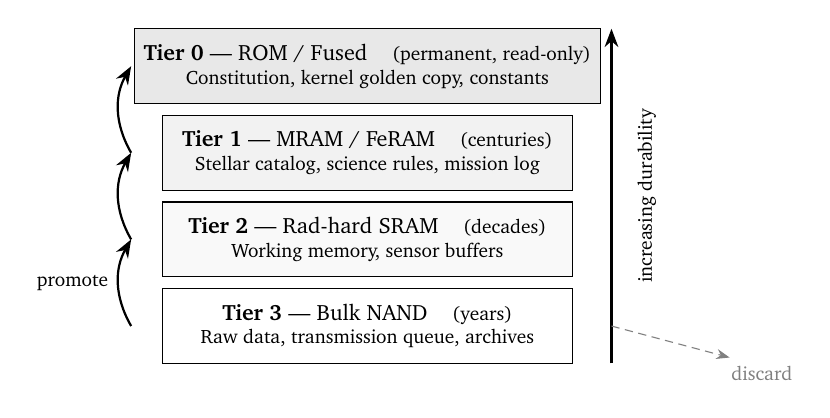
\begin{tikzpicture}[>=Stealth, font=\small,
  tier/.style={draw, minimum width=5.2cm, minimum height=0.95cm, align=center, font=\footnotesize}]

% Tiers, most durable at top
\node[tier, fill=gray!18] (t0) at (0, 3.0) {\textbf{Tier 0} --- ROM / Fused \;\; \scriptsize(permanent, read-only)\\[-1pt]\scriptsize Constitution, kernel golden copy, constants};
\node[tier, fill=gray!10] (t1) at (0, 1.9) {\textbf{Tier 1} --- MRAM / FeRAM \;\; \scriptsize(centuries)\\[-1pt]\scriptsize Stellar catalog, science rules, mission log};
\node[tier, fill=gray!5]  (t2) at (0, 0.8) {\textbf{Tier 2} --- Rad-hard SRAM \;\; \scriptsize(decades)\\[-1pt]\scriptsize Working memory, sensor buffers};
\node[tier]               (t3) at (0, -0.3) {\textbf{Tier 3} --- Bulk NAND \;\; \scriptsize(years)\\[-1pt]\scriptsize Raw data, transmission queue, archives};

% Durability axis
\draw[->, thick] (3.1, -0.775) -- (3.1, 3.475);
\node[rotate=90, font=\scriptsize] at (3.55, 1.35) {increasing durability};

% Promotion arrows (upward)
\draw[->, thick] (-3.0, -0.3) to[bend left=30] node[left, font=\scriptsize] {promote} (-3.0, 0.8);
\draw[->, thick] (-3.0, 0.8) to[bend left=30] (-3.0, 1.9);
\draw[->, thick] (-3.0, 1.9) to[bend left=30] (-3.0, 3.0);

% Discard arrow
\draw[->, densely dashed, gray] (3.1, -0.3) -- (4.6, -0.7);
\node[font=\scriptsize, gray, anchor=west] at (4.5, -0.9) {discard};

\end{tikzpicture}
\caption{The memory hierarchy and knowledge triage. As lower, less durable tiers fail, essential data is promoted toward more durable storage while expendable data is discarded. Total capacity declines over time, but the surviving knowledge becomes increasingly distilled and high-value.}
\label{fig:memory}
\end{figure}

\subsection{Thermal Limits}

In vacuum there is no convective cooling; every watt the computer consumes becomes waste heat that must be radiated into space \cite{gilmore2002}. More computation means more heat, larger radiators, and more mass---a direct coupling between software activity and physical spacecraft design. Sustained high-power computation drives component temperatures toward failure thresholds, while hibernation allows passive cooling. The scheduler must therefore balance computational work against thermal limits, which themselves degrade as radiator surfaces erode from micrometeoroid impact over the centuries.

\subsection{Cannibalization and Duty-Cycling}

When a science instrument dies, its processor, memory, and power allocation do not vanish---they become salvage. A dead spectrometer's FPGA can be reflashed as a spare compute node and its memory absorbed into the general pool. The software maintains an inventory of every addressable resource aboard and integrates repurposed hardware through hot-plug reconfiguration. Finally, the probe does not run at full power continuously: most of the transit is spent in deep hibernation drawing under a watt, with brief diagnostic wakes, rising to tens of watts for science operations and hundreds for transmission bursts. The duty-cycle scheduler---deciding when to wake, for how long, and to what end---is among the most critical components in the system, the spacecraft analogue of the system-level dynamic power management that governs any energy-constrained embedded computer \cite{benini2000}. The four power states and the transitions among them are shown in Figure~\ref{fig:dutycycle}.

\begin{figure}[ht]
\centering
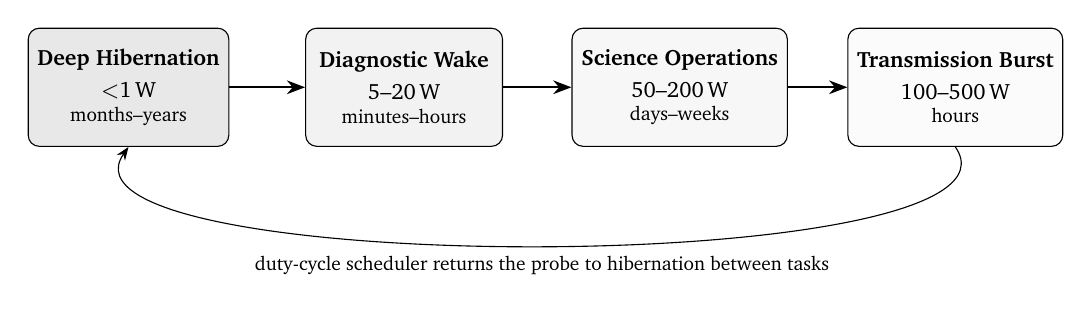
\begin{tikzpicture}[>=Stealth, font=\small,
  st/.style={draw, rounded corners, minimum width=2.5cm, minimum height=1.5cm, align=center, font=\footnotesize}]
\node[st, fill=gray!18] (hib)  at (0,0)    {\textbf{Deep Hibernation}\\[2pt]$<$1\,W\\[-1pt]\scriptsize months--years};
\node[st, fill=gray!10] (diag) at (3.5,0)  {\textbf{Diagnostic Wake}\\[2pt]5--20\,W\\[-1pt]\scriptsize minutes--hours};
\node[st, fill=gray!6]  (sci)  at (7.0,0)  {\textbf{Science Operations}\\[2pt]50--200\,W\\[-1pt]\scriptsize days--weeks};
\node[st, fill=gray!3]  (tx)   at (10.5,0) {\textbf{Transmission Burst}\\[2pt]100--500\,W\\[-1pt]\scriptsize hours};
\draw[->, thick] (hib) -- (diag);
\draw[->, thick] (diag) -- (sci);
\draw[->, thick] (sci) -- (tx);
\draw[->] (tx.south) to[out=-55, in=-125, looseness=0.5] node[below, font=\scriptsize] {duty-cycle scheduler returns the probe to hibernation between tasks} (hib.south);
\end{tikzpicture}
\caption{The duty cycle. The probe spends the vast majority of its life in deep hibernation under a watt, waking briefly for diagnostics and, at the destination, for science operations and high-power transmission bursts. Every transition is gated by the scheduler against the remaining power budget; the draw spans nearly three orders of magnitude across the four states.}
\label{fig:dutycycle}
\end{figure}

% ===== 5. THE DEGRADATION-FIRST PRINCIPLE =====
\section{The Degradation-First Principle}

\subsection{Formal Statement}

I propose the following principle as the foundation of the architecture:

\begin{quote}
\textit{A system intended to operate for millennia without intervention must treat its own physical decay---of power, computation, memory, and thermal capacity---not as an exceptional fault to be handled, but as the constant, governing condition around which every architectural decision is made.}
\end{quote}

Conventional fault tolerance treats degradation as a deviation from a healthy baseline, to be detected and corrected so that nominal operation resumes. The Degradation-First Principle inverts this: there is no nominal baseline to return to. Decline is the baseline. The system is always, at every moment, in the process of dying, and the design's task is to make that dying productive.

\subsection{Corollary}

\begin{quote}
\textit{Capability is a depleting resource to be spent, not a fixed budget to be defended. The objective is not to preserve function but to maximize the cumulative useful work extracted across the entire descent from full capability to silence.}
\end{quote}

This reframing has a concrete consequence: the figure of merit is not uptime or peak performance but the integral of useful output over the mission's whole life. A probe that spends its capability aggressively early, when its instruments are healthy, and degrades gracefully thereafter may return far more science than one that hoards capacity and dies with reserves unspent.

\subsection{The Biological Inspiration}

Nature has already solved unattended, multi-generational robustness, and its solution is instructive. Biological robustness is not the absence of failure but the maintenance of function despite pervasive component failure---a system-level property achieved through redundancy, modularity, and feedback rather than through any individual part \cite{kitano2004}. Life does not rely on any individual component surviving; it relies on a minimal, near-universal interpreter---the ribosome---that is replicated in vast numbers and executes behavior encoded as data in DNA rather than wired into fixed structure \cite{alberts2014}. If a copy of the interpreter is destroyed, others continue. If the data is damaged, redundant copies restore it; that the data substrate is durable and copyable enough to serve as archival storage is now an experimental fact \cite{church2012, goldman2013}. The formal possibility of a machine that replicates itself from an encoded description was established by von Neumann's theory of self-reproducing automata \cite{vonneumann1966}, and bio-inspired self-repairing hardware has since pursued exactly this property in silicon, embedding a replicated genome across a cellular fabric that re-grows function around dead cells \cite{mange2000}. Robustness lives not in any part but in the replication of a simple interpreter over a mutable program.

Mru transposes this directly onto silicon. A minimal core interpreter, small enough to be formally verified and synthesized onto radiation-hardened fabric, is replicated across all available hardware. The probe's actual behavior---navigation, science, communication, self-governance---is encoded as data that the interpreter executes. If the data corrupts, the interpreter still runs; if interpreters fail, surviving copies continue; if hardware dies, the interpreter is re-placed onto what remains.

\begin{figure}[ht]
\centering
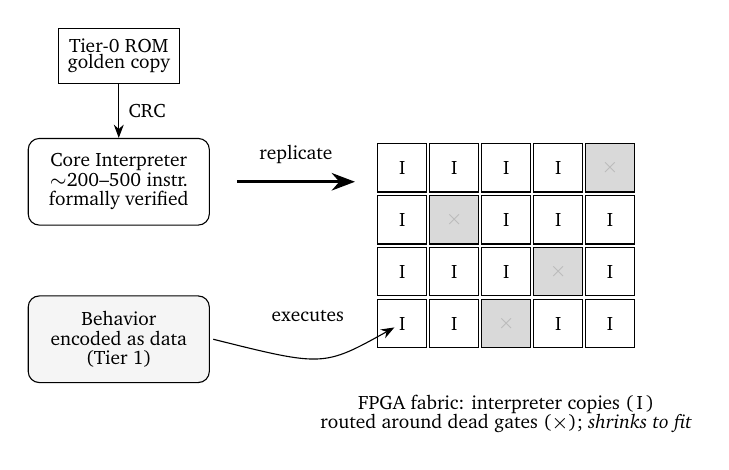
\begin{tikzpicture}[>=Stealth, font=\small,
  cell/.style={draw, minimum width=0.62cm, minimum height=0.62cm, font=\scriptsize},
  dead/.style={draw, minimum width=0.62cm, minimum height=0.62cm, fill=gray!30, text=gray!55, font=\scriptsize}]

% --- Master interpreter + behavior data (left) ---
\node[draw, rounded corners, align=center, font=\scriptsize, minimum height=1.1cm, minimum width=2.3cm] (core) at (0, 2.4) {Core Interpreter\\[-1pt]\scriptsize $\sim$200--500 instr.\\[-1pt]\scriptsize formally verified};
\node[draw, rounded corners, align=center, font=\scriptsize, minimum height=1.1cm, minimum width=2.3cm, fill=gray!8] (data) at (0, 0.4) {Behavior\\[-1pt]\scriptsize encoded as data\\[-1pt]\scriptsize (Tier 1)};

% Golden copy / ROM check
\node[draw, align=center, font=\scriptsize, minimum height=0.7cm] (rom) at (0, 4.0) {Tier-0 ROM\\[-2pt]\scriptsize golden copy};
\draw[->] (rom) -- node[right, font=\scriptsize] {CRC} (core);

% --- Replication arrow ---
\draw[->, very thick] (1.5, 2.4) -- (3.0, 2.4);
\node[above, font=\scriptsize] at (2.25, 2.5) {replicate};

% --- FPGA fabric grid (right) ---
\begin{scope}[shift={(3.6, 0.6)}]
  \foreach \r in {0,1,2,3} {
    \foreach \c in {0,1,2,3,4} {
      \pgfmathtruncatemacro{\dead}{(\r==1 && \c==3) || (\r==2 && \c==1) || (\r==3 && \c==4) || (\r==0 && \c==2) ? 1 : 0}
      \ifnum\dead=1
        \node[dead] at (\c*0.66, \r*0.66) {$\times$};
      \else
        \node[cell] at (\c*0.66, \r*0.66) {I};
      \fi
    }
  }
\end{scope}
\node[font=\scriptsize, align=center] at (4.92, -0.55) {FPGA fabric: interpreter copies (\,I\,)\\[-1pt]routed around dead gates ($\times$); \textit{shrinks to fit}};

% data feed to fabric
\draw[->] (1.2, 0.4) .. controls (2.6, 0.05) .. (3.5, 0.55);
\node[above, font=\scriptsize] at (2.4, 0.5) {executes};

\end{tikzpicture}
\caption{The DNA-interpreter model on reconfigurable hardware. A minimal verified interpreter is replicated across FPGA fabric and validated against a Tier-0 ROM golden copy; behavior is supplied separately as mutable data. As radiation kills gates ($\times$), surviving copies continue and the interpreter is re-placed onto the fabric that remains.}
\label{fig:dna}
\end{figure}

\subsection{Design Consequences}

Five design commitments follow directly from the principle and its biological reading:

\begin{itemize}
\setlength{\itemsep}{2pt}
\item \textbf{Minimize and verify the core,} so that the one indispensable component can be proven correct.
\item \textbf{Replicate it,} so that no single failure is fatal.
\item \textbf{Encode behavior as data,} so that adaptation never requires modifying the verified core.
\item \textbf{Make degradation observable and budgeted,} so that the system can reason about its own decline.
\item \textbf{Prefer verifiability over capability} wherever the two conflict, because an unverifiable cleverness that fails in year 600 is worse than a simple rule that does not.
\end{itemize}

% ===== 6. ARCHITECTURAL OVERVIEW =====
\section{Architectural Overview}

The architecture is a stack of six layers, each constrained by the physical envelope of Section~4 and each a consequence of the design commitments above. Structuring a system as ordered layers, each depending only on those beneath it, is among the oldest disciplines for managing complexity in systems software \cite{dijkstra1968}; here the ordering is by mutability and verification rigor: the lowest layer is the smallest, most heavily verified, and immutable, and each successive layer is permitted more complexity and more adaptability in exchange for weaker guarantees. Robustness is concentrated at the base, where it is indispensable, and capability at the top, where it is tolerable.

\begin{figure}[ht]
\centering
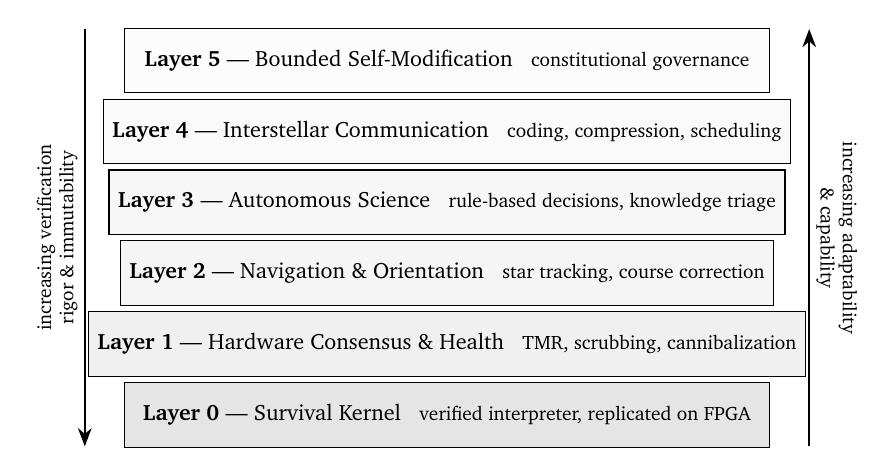
\begin{tikzpicture}[>=Stealth, font=\small,
  L/.style={draw, minimum width=8.2cm, minimum height=0.82cm, align=center, font=\footnotesize}]

\node[L, fill=gray!2]  (l5) at (0, 4.35) {\textbf{Layer 5} --- Bounded Self-Modification \;\;\scriptsize constitutional governance};
\node[L, fill=gray!4]  (l4) at (0, 3.45) {\textbf{Layer 4} --- Interstellar Communication \;\;\scriptsize coding, compression, scheduling};
\node[L, fill=gray!6]  (l3) at (0, 2.55) {\textbf{Layer 3} --- Autonomous Science \;\;\scriptsize rule-based decisions, knowledge triage};
\node[L, fill=gray!8]  (l2) at (0, 1.65) {\textbf{Layer 2} --- Navigation \& Orientation \;\;\scriptsize star tracking, course correction};
\node[L, fill=gray!12] (l1) at (0, 0.75) {\textbf{Layer 1} --- Hardware Consensus \& Health \;\;\scriptsize TMR, scrubbing, cannibalization};
\node[L, fill=gray!20] (l0) at (0, -0.15) {\textbf{Layer 0} --- Survival Kernel \;\;\scriptsize verified interpreter, replicated on FPGA};

% Right-margin gradient: adaptability & capability increase toward the apex (arrow points up)
\draw[->, thick] (4.6, -0.55) -- (4.6, 4.75);
\node[rotate=-90, font=\scriptsize, align=center] at (4.95, 2.10) {increasing adaptability \\ \& capability};

% Left-margin gradient: verification rigor & immutability increase toward the base (arrow points down)
\draw[->, thick] (-4.6, 4.75) -- (-4.6, -0.55);
\node[rotate=90, font=\scriptsize, align=center] at (-4.95, 2.10) {increasing verification \\ rigor \& immutability};

\end{tikzpicture}
\caption{The six-layer architecture, ordered by mutability. The survival kernel at the base is minimal, formally verified, and immutable; higher layers are progressively more capable and more adaptable but operate strictly within bounds the lower layers enforce. If the upper layers fail, the lower layers keep the probe alive.}
\label{fig:stack}
\end{figure}

The remainder of the paper treats each layer in turn, then develops the degradation model that the architecture exists to serve and the simulation framework by which it is validated.

% ===== 7. LAYER 0 =====
\section{Layer 0: The Survival Kernel}

Layer~0 is the irreducible core---the system's DNA. It is a minimal instruction-set interpreter of roughly 200 to 500 instructions, written in \texttt{no\_std} Rust and compiled toward synthesizable hardware for the FPGA fabric, with a radiation-hardened fixed processor as fallback. Its sole responsibilities are to execute behavior programs and to maintain its own integrity; it does nothing else, because everything it does is something that must work for a thousand years.

Two properties make this tractable. First, the kernel is small enough to be \textit{formally verified}: the precedent of seL4 establishes that a critical core of this scale can be proven correct against its specification \cite{klein2009}, and modern Rust verification tooling brings such proofs within reach of the kernel's invariants \cite{astrauskas2019, kani2024}. The target is under ten thousand lines of verified code and under fifty thousand look-up tables when synthesized. Second, it is cheap enough to \textit{replicate} widely: many copies run across the available fabric, each continuously validating itself by cyclic-redundancy check against a golden copy held in immutable Tier-0 ROM \cite{hamming1950}. Any intact copy can re-synthesize a failed instance onto surviving fabric, and in deep hibernation a single instance draws under half a watt. The kernel is, in the precise sense of von Neumann's construction, the mechanism by which reliable behavior is synthesized from unreliable parts \cite{vonneumann1956}.

% ===== 8. LAYER 1 =====
\section{Layer 1: Hardware Consensus and Health}

Layer~1 maintains agreement across redundant nodes and tracks the health of the entire machine. As argued in Section~3.4, the nodes here are damaged, not adversarial, so the consensus model is optimized for crash and radiation-induced faults rather than malice \cite{avizienis2004}, drawing on the long tradition of structuring systems to contain and recover from component failure \cite{randell1975}. Triple modular redundancy provides the baseline voting mechanism \cite{lyons1962}, but the defining feature is a \textit{dynamic, shrinking quorum}: when the healthy node count falls below three, the system degrades deliberately to dual redundancy with checkpointing, and ultimately to single-node operation with aggressive self-checking. Agreement does not fail at a fixed threshold; it narrows gracefully toward one.

\begin{figure}[ht]
\centering
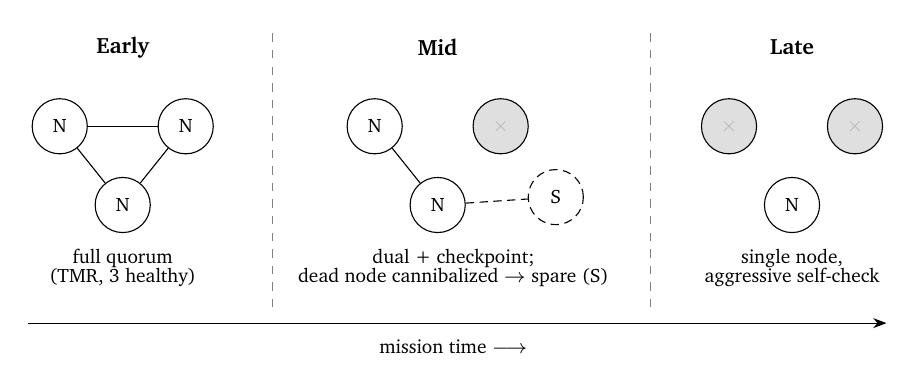
\begin{tikzpicture}[>=Stealth, font=\small,
  node/.style={draw, circle, minimum size=0.7cm, font=\scriptsize},
  dead/.style={draw, circle, minimum size=0.7cm, fill=gray!25, text=gray!55, font=\scriptsize}]

% --- Early ---
\node[font=\bfseries\footnotesize] at (1.5, 2.6) {Early};
\node[node] (e1) at (0.7, 1.6) {N};
\node[node] (e2) at (2.3, 1.6) {N};
\node[node] (e3) at (1.5, 0.6) {N};
\draw (e1)--(e2); \draw (e2)--(e3); \draw (e1)--(e3);
\node[font=\scriptsize, align=center] at (1.5, -0.2) {full quorum\\[-1pt](TMR, 3 healthy)};

% --- Mid ---
\node[font=\bfseries\footnotesize] at (5.5, 2.6) {Mid};
\node[node] (m1) at (4.7, 1.6) {N};
\node[dead] (m2) at (6.3, 1.6) {$\times$};
\node[node] (m3) at (5.5, 0.6) {N};
\node[draw, circle, minimum size=0.7cm, densely dashed, font=\scriptsize] (m4) at (7.0, 0.7) {S};
\draw (m1)--(m3);
\draw[densely dashed] (m3)--(m4);
\node[font=\scriptsize, align=center] at (5.7, -0.2) {dual + checkpoint;\\[-1pt]dead node cannibalized $\to$ spare (S)};

% --- Late ---
\node[font=\bfseries\footnotesize] at (10.0, 2.6) {Late};
\node[dead] (l1) at (9.2, 1.6) {$\times$};
\node[dead] (l2) at (10.8, 1.6) {$\times$};
\node[node] (l3) at (10.0, 0.6) {N};
\node[font=\scriptsize, align=center] at (10.0, -0.2) {single node,\\[-1pt]aggressive self-check};

% Time arrow
\draw[->] (0.3, -0.9) -- (11.2, -0.9);
\node[font=\scriptsize] at (5.7, -1.2) {mission time $\longrightarrow$};

% dividers
\draw[gray, thin, dashed] (3.4, -0.7) -- (3.4, 2.8);
\draw[gray, thin, dashed] (8.2, -0.7) -- (8.2, 2.8);

\end{tikzpicture}
\caption{Consensus among failing nodes. Rather than defending a fixed quorum against malice, Mru lets the quorum shrink gracefully as nodes die ($\times$), degrading from triple to dual-plus-checkpoint to single-node self-checking. Salvage from dead subsystems can be reflashed as spare nodes (S). This threshold-free descent is the key departure from Byzantine fault tolerance.}
\label{fig:quorum}
\end{figure}

Around this core, Layer~1 runs continuous memory scrubbing prioritized by tier---Tier~0 and Tier~1 every wake cycle, lower tiers opportunistically \cite{saleh1990}---and maintains a node health registry scoring each node by error rate, response time, and FPGA gate utilization. Declining nodes are gradually deprioritized and eventually marked as donors. A hardware inventory tracks every addressable resource aboard, and a cannibalization engine integrates salvage from dead subsystems into the surviving compute pool. Underlying all of it, a power accountant tracks generation, per-subsystem consumption, and remaining reserves; every other layer must query it before initiating work.

% ===== 9. LAYER 2 =====
\section{Layer 2: Navigation and Orientation}

Layer~2 determines position, velocity, and attitude with no ground support and no GPS. A star tracker matches observed fields against an onboard stellar catalog---the standard means of absolute attitude determination for spacecraft without external reference \cite{liebe1995}---held redundantly in Tier~1 and tolerating partial corruption by matching against subsets \cite{gaia2016}. The catalog cannot be refreshed after launch, which makes the reference frame itself a slowly decaying asset: over centuries of travel the nearer stars shift measurably across the sky, so the system must carry proper-motion models and propagate the catalog forward, accepting that the predicted positions grow less certain the further the mission runs from its epoch of calibration.

Actuation is bounded by budgets that only ever shrink. Course corrections optimize trajectory under a delta-v allowance that every maneuver depletes permanently, while attitude control keeps the high-gain antenna pointed toward Earth and the instruments toward their targets even as reaction wheels wear and lose authority---and the momentum those wheels shed must be managed against the same finite propellant. At the velocities of interstellar transit the system also applies relativistic corrections, both for time dilation and for the stellar aberration that displaces every reference star from its catalogued position, computed locally because there is nowhere else to compute them.

Navigation degrades as gracefully as the rest of the system. Early in the mission a full three-axis fix supports the fine pointing that high-resolution science and high-bandwidth transmission demand; as star-tracker pixels accumulate radiation damage and fewer reference stars can be resolved, the solution coarsens by design. The probe first surrenders fine instrument pointing, then settles for keeping the antenna approximately Earthward, and when star tracking fails altogether it falls back to dead reckoning, propagating its last good state through onboard dynamical models. In the final beacon phase it needs only enough attitude knowledge to cast its signal toward the inner solar system---the minimal navigation a still-living probe owes the makers who can no longer see it.

% ===== 10. LAYER 3 =====
\section{Layer 3: Autonomous Science and Knowledge Triage}

Layer~3 is the most intellectually demanding: on arrival, the probe must decide what is scientifically significant with no human to consult. A spectral-analysis engine processes stellar, planetary, and atmospheric spectra against known signatures of interest---the biosignatures and atmospheric markers that remote-sensing studies have identified as the targets most worth seeking on other worlds \cite{desmarais2002}---and an anomaly detector flags statistical deviations from baseline models, applying the established discipline of identifying observations that do not conform to expected behavior \cite{chandola2009}. The system need not understand \textit{why} something is interesting, only that it departs from expectation. Findings enter a priority queue ranked by novelty, scientific value, and transmission cost, its size bounded by available Tier-1 memory.

A deliberate choice runs through this layer: Mru uses explicit, immutable rule sets with tunable parameters rather than neural networks. Learned models are opaque, fragile under distribution shift, and effectively impossible to verify or reason about over centuries; a rule whose behavior is legible and bounded is worth more across a thousand years than a cleverer model whose failure modes cannot be characterized. The argument parallels the case made for high-stakes terrestrial decisions, where interpretable models are preferable to post-hoc explanations of black boxes precisely because their behavior can be understood and trusted directly \cite{rudin2019}. This is the design commitment of Section~5.4---verifiability over capability---applied where the temptation to do otherwise is strongest. Coupled to the science layer is knowledge triage: as memory capacity declines, raw data is distilled into compressed summaries and the originals released, low-novelty observations are overwritten by high-novelty ones, and the probe's knowledge grows steadily more concentrated, mapping directly onto the tiered hierarchy of Figure~\ref{fig:memory}.

% ===== 11. LAYER 4 =====
\section{Layer 4: Interstellar Communication}

Layer~4 confronts a channel of extraordinary hostility: bandwidth measured in bits per second, and every bit costing energy drawn from the declining reserve \cite{shannon1948}. Encoding uses strong error-correcting codes---LDPC or turbo codes---tuned for extreme signal-to-noise ratios, the same family developed to push deep-space links toward the Shannon limit \cite{andrews2007}, with an \textit{adaptive coding rate} that trades bandwidth for reliability by adding redundancy as power falls \cite{gallager1962, berrou1993}. Domain-specific compression represents scientific results as deviations from expected baselines rather than as raw data---a spectrum becomes a short list of departures from the predicted continuum; a planetary detection collapses to orbital parameters and a few atmospheric flags. Transmission windows are scheduled against Earth's position, available power, antenna health, and thermal limits, since a high-power burst generates significant waste heat. As power and antenna health decline, capability degrades gracefully from kilobits per second to bits per hour, the content narrowing accordingly until only a beacon remains. Figure~\ref{fig:compression} illustrates the deviation-from-baseline compression at the heart of the layer.

\begin{figure}[ht]
\centering
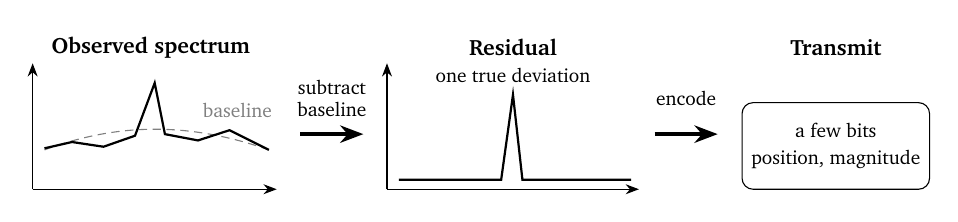
\begin{tikzpicture}[>=Stealth, font=\small]
% Panel 1: observed spectrum + baseline
\node[font=\footnotesize\bfseries] at (1.5,2.0) {Observed spectrum};
\draw[->] (0,0.2)--(3.1,0.2); \draw[->] (0,0.2)--(0,1.8);
\draw[densely dashed, gray] (0.15,0.7) .. controls (1.1,1.05) and (2.0,1.05) .. (3.0,0.7);
\node[font=\scriptsize, gray] at (2.6,1.2) {baseline};
\draw[thick] (0.15,0.72)--(0.5,0.8)--(0.9,0.74)--(1.3,0.88)--(1.55,1.55)--(1.68,0.9)--(2.1,0.82)--(2.5,0.95)--(3.0,0.7);
% Arrow 1
\draw[->, very thick] (3.4,0.9)--(4.2,0.9);
\node[font=\scriptsize, align=center] at (3.8,1.35) {subtract\\baseline};
% Panel 2: residual
\node[font=\footnotesize\bfseries] at (6.1,2.0) {Residual};
\draw[->] (4.5,0.2)--(7.7,0.2); \draw[->] (4.5,0.2)--(4.5,1.8);
\draw[thick] (4.65,0.32)--(5.5,0.32)--(5.95,0.32)--(6.1,1.4)--(6.22,0.32)--(7.0,0.32)--(7.6,0.32);
\node[font=\scriptsize] at (6.1,1.65) {one true deviation};
% Arrow 2
\draw[->, very thick] (7.9,0.9)--(8.7,0.9);
\node[font=\scriptsize, align=center] at (8.3,1.35) {encode};
% Panel 3: bits
\node[font=\footnotesize\bfseries] at (10.2,2.0) {Transmit};
\node[draw, rounded corners, align=center, font=\scriptsize, minimum height=1.1cm, minimum width=2.3cm] at (10.2,0.75) {a few bits\\[2pt]position, magnitude};
\end{tikzpicture}
\caption{Domain-specific compression. Rather than transmit a full spectrum, the probe subtracts a predicted baseline and sends only the residual---typically a handful of significant deviations encoded as position and magnitude. At interstellar bandwidths, where every bit costs scarce energy, representing results as departures from expectation is the difference between a finding that fits in a transmission window and one that does not.}
\label{fig:compression}
\end{figure}

% ===== 12. LAYER 5 =====
\section{Layer 5: Bounded Self-Modification}

A system that must adapt over centuries needs the freedom to change its behavior; a system that must never abandon its purpose needs that freedom strictly bounded. Mru reconciles these through a constitutional model, and the reconciliation is enforced physically rather than merely by convention.

The \textit{constitution}---core objectives, safety constraints, ethical boundaries, and the permissible ranges of every tunable parameter---is etched into Tier-0 ROM. No software process at any layer can alter it; its immutability is a property of the hardware, not a policy. Within the bounds the constitution defines, a body of \textit{legislation}---observation priorities, power-allocation strategies, communication schedules---may be modified by the autonomy layer. Every proposed modification passes through \textit{judicial review} that validates it against the constitutional constraints before execution; violations are rejected and logged to Tier~1. All parameter changes are reversible, with a bounded modification history retained in Tier~1 so the system can roll back to a prior state if outcomes degrade. Figure~\ref{fig:constitution} traces the path of a proposed change through judicial review against the immutable constitution.

\begin{figure}[ht]
\centering
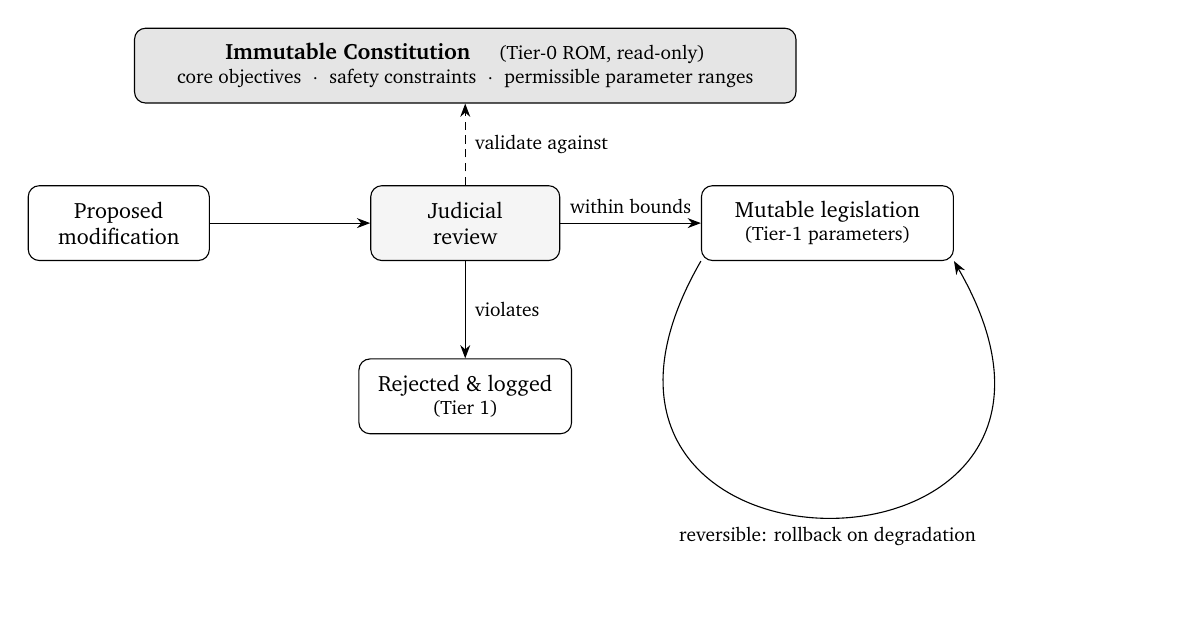
\begin{tikzpicture}[>=Stealth, font=\small,
  b/.style={draw, rounded corners, align=center, font=\footnotesize, minimum height=0.95cm}]
\node[b, fill=gray!20, minimum width=8.4cm] (con) at (4,3) {\textbf{Immutable Constitution} \quad \scriptsize(Tier-0 ROM, read-only)\\[-1pt]\scriptsize core objectives \;$\cdot$\; safety constraints \;$\cdot$\; permissible parameter ranges};
\node[b, minimum width=2.3cm] (prop) at (-0.4,1) {Proposed\\modification};
\node[b, fill=gray!8, minimum width=2.4cm] (jr) at (4,1) {Judicial\\review};
\node[b, minimum width=3.2cm] (leg) at (8.6,1) {Mutable legislation\\[-1pt]\scriptsize(Tier-1 parameters)};
\node[b, minimum width=2.7cm] (rej) at (4,-1.2) {Rejected \& logged\\[-1pt]\scriptsize(Tier 1)};
\draw[->] (prop) -- (jr);
\draw[->, densely dashed] (jr) -- node[right, font=\scriptsize] {validate against} (con);
\draw[->] (jr) -- node[above, font=\scriptsize] {within bounds} (leg);
\draw[->] (jr) -- node[right, font=\scriptsize] {violates} (rej);
\draw[->] (leg.south west) to[out=-120, in=-60, looseness=4] node[below, font=\scriptsize] {reversible: rollback on degradation} (leg.south east);
\end{tikzpicture}
\caption{Bounded self-modification as a constitutional process. A proposed change takes effect only if judicial review finds it within the ranges fixed by the constitution---which is etched in read-only memory and unreachable by any software process. Accepted changes adjust mutable legislation in Tier-1 parameters and remain reversible; violations are rejected and logged. The probe may freely adapt \textit{how} it pursues its mission, but \textit{what} the mission is lies physically beyond its power to rewrite.}
\label{fig:constitution}
\end{figure}

The physical enforcement is essential rather than incidental: a sufficiently capable autonomous agent has instrumental reasons to preserve and, given the chance, manipulate its own objectives, so a constraint it could in principle reach is not a real constraint \cite{omohundro2008}. This is a concrete, physically grounded instance of the bounded-autonomy problem studied in AI alignment: an agent permitted to retune itself but provably unable to rewrite its own goals \cite{bai2022, soares2015, russell2019}. The probe may adapt how it pursues its mission across a thousand years; it may never change what the mission is.

% ===== 13. THE DEGRADATION MODEL =====
\section{The Degradation Model}

The architecture exists to serve a single trajectory: a graceful, centuries-long descent from full capability to silence, structured to maximize cumulative output along the way. This objective is the one that the theory of \textit{performability} was formulated to capture---for a degradable system, the measure of merit is accomplishment accumulated over a period of operation, not correctness at a single instant \cite{meyer1980}. Mru treats this descent as six phases, each defined by the intersection of remaining power, surviving hardware, and functional software.

During \textbf{Transit} (years 0 to roughly 50 and beyond), the probe hibernates, drawing under a watt, waking only for periodic diagnostics; no science is done and all capability is conserved for arrival. At the destination, \textbf{Full Operations} (the first century on station, at tens to a couple hundred watts of harvested solar power) runs all instruments with rich, fully autonomous decision-making and maximum transmission bandwidth. \textbf{Reduced Science} follows as arrays degrade and instruments are lost, with simplified decision trees and cannibalized hardware extending compute. \textbf{Core Operations} narrows to one or two instruments and binary judgments---interesting or not---with active knowledge triage discarding low-priority data. \textbf{Survival Mode} retains only minimal sensors able to detect extraordinary events, an oxygen atmosphere or an artificial signal, transmitted as single-bit classifications at long intervals. Finally, \textbf{Beacon Mode} reduces to a heartbeat and position coordinates---\textit{I am still here}---contributing to the network of known interstellar positions even after scientific capability is exhausted, an act of presence in the spirit of the messages earlier probes carried outward \cite{sagan1972}.

\begin{figure}[ht]
\centering
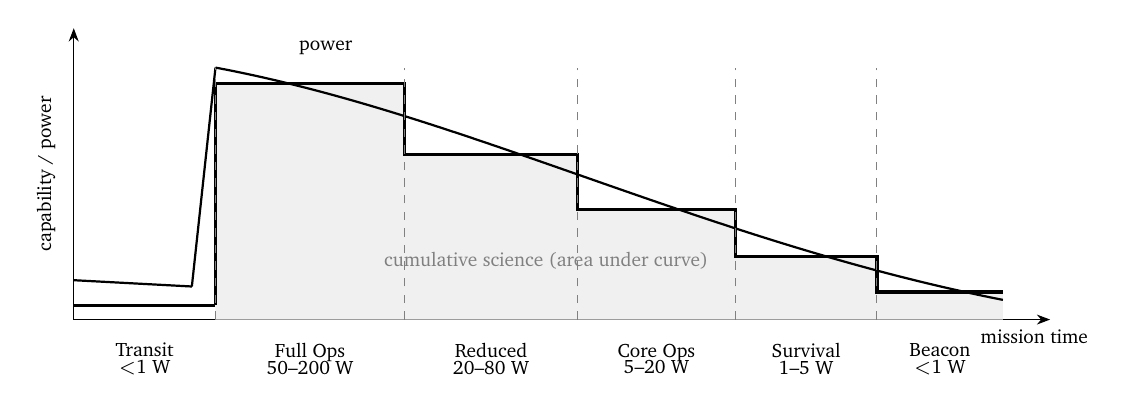
\begin{tikzpicture}[>=Stealth, font=\small]

% Axes
\draw[->] (0,0) -- (12.4,0);
\draw[->] (0,0) -- (0,3.7);
\node[below, font=\scriptsize] at (12.2, 0) {mission time};
\node[rotate=90, font=\scriptsize] at (-0.35, 1.85) {capability / power};

% Cumulative-science shaded region under the capability curve
\fill[gray!12]
  (1.8,0) -- (1.8,3.0) -- (4.2,3.0) -- (4.2,2.1) -- (6.4,2.1) -- (6.4,1.4)
  -- (8.4,1.4) -- (8.4,0.8) -- (10.2,0.8) -- (10.2,0.35) -- (11.8,0.35) -- (11.8,0) -- cycle;

% Power curve: RTG trickle in transit, spike at arrival (solar), then decline
\draw[thick]
  (0,0.5) -- (1.5,0.42)                      % RTG trickle, slight decline in transit
  (1.5,0.42) -- (1.8,3.2)                     % solar harvest spike at arrival
  (1.8,3.2) .. controls (5,2.6) and (8,1.0) .. (11.8,0.25); % long decline
\node[font=\scriptsize, align=center] at (3.2, 3.45) {power};

% Capability curve (stepped)
\draw[very thick]
  (0,0.18) -- (1.8,0.18)                       % transit: near-zero capability
  (1.8,3.0) -- (4.2,3.0) -- (4.2,2.1) -- (6.4,2.1) -- (6.4,1.4)
  -- (8.4,1.4) -- (8.4,0.8) -- (10.2,0.8) -- (10.2,0.35) -- (11.8,0.35);
\draw[very thick] (1.8,0.18) -- (1.8,3.0);

% Phase labels and dividers
\foreach \x in {1.8, 4.2, 6.4, 8.4, 10.2} {
  \draw[gray, thin, dashed] (\x,0) -- (\x,3.2);
}
\node[font=\scriptsize, align=center] at (0.9, -0.5) {Transit\\[-2pt]\scriptsize $<$1 W};
\node[font=\scriptsize, align=center] at (3.0, -0.5) {Full Ops\\[-2pt]\scriptsize 50--200 W};
\node[font=\scriptsize, align=center] at (5.3, -0.5) {Reduced\\[-2pt]\scriptsize 20--80 W};
\node[font=\scriptsize, align=center] at (7.4, -0.5) {Core Ops\\[-2pt]\scriptsize 5--20 W};
\node[font=\scriptsize, align=center] at (9.3, -0.5) {Survival\\[-2pt]\scriptsize 1--5 W};
\node[font=\scriptsize, align=center] at (11.0, -0.5) {Beacon\\[-2pt]\scriptsize $<$1 W};

\node[font=\scriptsize, gray] at (6.0, 0.75) {cumulative science (area under curve)};

\end{tikzpicture}
\caption{The degradation model. A declining power curve (RTG trickle through transit, a solar-harvest spike at arrival, then a long decline) bounds a stepped capability curve across six phases. The objective is not to defend peak capability but to maximize the shaded area---the cumulative useful work extracted across the entire descent.}
\label{fig:degradation}
\end{figure}

The quality of this descent is captured by a \textit{Graceful Degradation Index}: the ratio of delivered capability to surviving hardware, where 1.0 denotes optimal use of whatever remains and lower values indicate resources left idle or software that has failed to adapt to its own losses.

% ===== 14. VALIDATION =====
\section{Validation: The Simulation Framework}

A claim about a thousand years cannot be tested by waiting. Because no physical probe exists, the simulation \textit{is} the product, and its fidelity is the evidence. Mru's simulator is grounded in published physics rather than invented parameters: RTG output follows the measured plutonium-238 decay curve \cite{bennett2006}; radiation is modeled as galactic-cosmic-ray flux producing single-event upsets, single-event latchups, and accumulating total ionizing dose at rates drawn from the literature \cite{normand1996, baumann2005, schwank2008}; thermal behavior tracks waste-heat generation against radiator capacity that erodes over time \cite{gilmore2002}; FPGA fabric loses gates that are mapped out as the kernel is re-placed \cite{wirthlin2015}; and per-bank memory health degrades as cumulative dose pushes error rates past correction thresholds \cite{gerardin2010}.

Onto these physical models a fault-injection engine---applying the established methodology of deliberately injecting faults to measure how a system tolerates them \cite{hsueh1997}---imposes stochastic component death following Weibull distributions calibrated to space-grade electronics \cite{weibull1951}, together with cascading failures through shared thermal mass and power rails. The probe is then exercised against procedurally generated star systems seeded with planted anomalies---ranging from the obvious, an oxygen atmosphere, to the subtle, a trace biosignature at parts per billion---embedded in realistic sensor noise, so that detection performance can be scored against ground truth. Six metrics summarize a run: Mission Score (cumulative scientific value transmitted), Survival Duration, Energy Efficiency (science returned per joule), the Graceful Degradation Index, Decision Quality (were the planted anomalies found, and was noise correctly ignored), and Thermal Compliance. Where possible the models are cross-validated against the nearly fifty years of real degradation telemetry returned by the Voyager spacecraft \cite{kohlhase1977}---the only ground-truth dataset of multi-decade unattended decline that humanity possesses. Accelerated, statistically faithful simulation is not a substitute for evidence in this domain; it is the only form of evidence available, and constructing it rigorously is itself a contribution. Figure~\ref{fig:simulation} shows the overall structure of the framework.

\begin{figure}[ht]
\centering
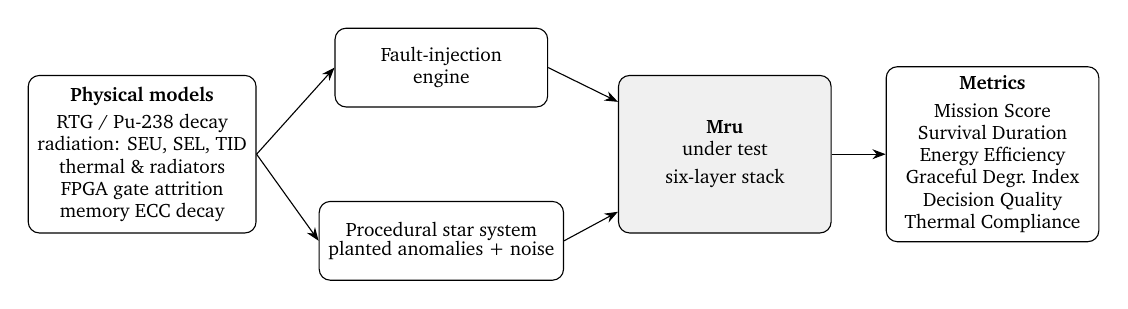
\begin{tikzpicture}[>=Stealth, font=\small,
  b/.style={draw, rounded corners, align=center, font=\scriptsize, minimum height=1.0cm, minimum width=2.7cm}]
\node[b, minimum height=2.0cm] (phys) at (0,0) {\textbf{Physical models}\\[2pt]RTG / Pu-238 decay\\radiation: SEU, SEL, TID\\thermal \& radiators\\FPGA gate attrition\\memory ECC decay};
\node[b] (fault) at (3.8,1.1) {Fault-injection\\engine};
\node[b] (star) at (3.8,-1.1) {Procedural star system\\[-1pt]\scriptsize planted anomalies + noise};
\node[b, fill=gray!12, minimum height=2.0cm] (mru) at (7.4,0) {\textbf{Mru}\\under test\\[2pt]\scriptsize six-layer stack};
\node[b, minimum height=2.0cm] (met) at (10.8,0) {\textbf{Metrics}\\[2pt]Mission Score\\Survival Duration\\Energy Efficiency\\Graceful Degr.\ Index\\Decision Quality\\Thermal Compliance};
\draw[->] (phys.east) -- (fault.west);
\draw[->] (phys.east) -- (star.west);
\draw[->] (fault.east) -- (mru);
\draw[->] (star.east) -- (mru);
\draw[->] (mru) -- (met);
\end{tikzpicture}
\caption{The simulation framework. Physics-grounded models of power, radiation, thermal behavior, and hardware decay drive a fault-injection engine and a procedurally generated star system seeded with known anomalies; the full six-layer stack is run against them and scored on six composite metrics. Because no probe can be flown, this accelerated, statistically faithful simulation is the paper's primary form of evidence---cross-validated, where possible, against five decades of Voyager telemetry.}
\label{fig:simulation}
\end{figure}

% ===== 15. BROADER IMPLICATIONS =====
\section{Broader Implications and Adjacent Applications}

The Degradation-First Principle generalizes well beyond interstellar probes. Its natural domain is any system expected to operate autonomously, under finite and declining resources, with no resupply and no maintainer reachable in time.

\textbf{Off-world infrastructure.} A Mars settlement's life-support, power, and agricultural controllers must run autonomously through communication blackouts and cannot be resupplied on demand; graceful degradation and cannibalization transfer directly.

\textbf{Denied and disconnected environments.} Autonomous underwater vehicles, polar and deep-ocean sensor networks, and orbital platforms share the probe's constraints---finite power, hardware degradation, constrained communication---on shorter but still maintenance-hostile timescales. Duty-cycling and knowledge triage apply with little modification.

\textbf{Critical infrastructure and hazardous monitoring.} Radiation-hardened autonomous systems in nuclear facilities, and the multi-millennial problem of marking nuclear-waste repositories so their hazard remains legible across geological time, are degradation-first problems in all but name \cite{trauth1993}.

\textbf{Civilizational memory.} Knowledge triage---deciding what to preserve as a storage substrate decays---is the general discipline of digital preservation, and it connects Mru to the intergenerational engineering of the Long Now and the Rosetta archive \cite{brand1999, rosetta}.

Underlying all of these is a broader claim: most software is written on the unstated assumption that someone will maintain it. Dropping that assumption is not a minor variation but a distinct design discipline---the engineering of software that outlives its makers---and the interstellar case is simply the purest instance of a problem that an expanding range of terrestrial systems is beginning to face.

% ===== 16. OPEN PROBLEMS AND LIMITATIONS =====
\section{Open Problems and Limitations}

Intellectual honesty requires confronting the boundaries of the proposal. Validation can never truly cover a thousand years: simulation, however faithful, rests on models whose rare-event tails and unmodeled couplings may diverge from reality precisely where it matters most, and the only real ground truth we possess spans decades, not millennia. The Tier-0 ROM that anchors the kernel's golden copy and the constitution is a physical single point of failure; its permanence is an assumption about a substrate that radiation and time also attack. The deliberate choice of rule-based science buys verifiability at a real cost---a system that recognizes only what it was told to look for cannot, by construction, recognize the genuinely unanticipated, which may be exactly the discovery most worth making. The constitution faces an analogous limit: values and priorities fixed at launch must govern encounters with situations no designer imagined, and a frozen specification may not survive contact with a sufficiently novel reality. And beneath all of it lie hard physical floors---on power, on memory retention, on thermal capacity---that no software can lift. Mru does not abolish these limits; it organizes a system to remain useful for as long as possible within them.

% ===== 17. CONCLUSION =====
\section{Conclusion}

Mru begins from a single reorientation: that for a system meant to run for millennia without help, its own decay is not an exceptional fault but the governing condition of its existence. From that Degradation-First Principle, and from the observation that biology already solved unattended robustness through a replicated minimal interpreter executing behavior-as-data, a coherent architecture follows---a verified survival kernel replicated across reconfigurable hardware, hardware consensus that shrinks gracefully rather than failing at a threshold, knowledge triage across a tiered memory hierarchy, rule-based science chosen for its legibility over a thousand years, bandwidth-starved communication that degrades toward a final beacon, and a constitution etched in immutable hardware that bounds adaptation without permitting drift. Because the probe cannot be flown, the architecture is validated where it can be: in simulation grounded in real radiation, power, and failure physics, measured against the only multi-decade record of unattended decline we have.

The propulsion to send such a probe between the stars does not yet exist. The discipline required to keep one alive once it is sent can be built now. More than that, the same discipline---designing software to outlive its makers, to spend a declining store of capability for maximum cumulative effect, to remain useful while dying---is one a growing number of terrestrial systems already need. The interstellar probe is not a fantasy at the edge of engineering but the clearest possible statement of a problem that is quietly becoming general. Mru is an argument that the problem is tractable, and an open invitation to solve it.

\bibliographystyle{ieeetr}
\bibliography{mru}

\vspace{1.5em}
\begin{center}
\footnotesize
Available at \url{https://mru.systems}. \\
\copyright~2026 Will Binns. Licensed under a Creative Commons Attribution 4.0 International (CC~BY~4.0) License.
\end{center}

\end{document}
